\chapter{Algoritmo MOPSO-hv}

  En este c\'apitulo se describe el algoritmo de c\'umulo de part\'iculas multi-objetivo propuesto en este trabajo 
  de tesis. Dicho algoritmo tiene un mecanismo de selecci\'on basado en la contribuci\'on al hipervolumen y adopta un operador de turbulencia.
  El algoritmo propuesto, se denomin\'o \textit{multi-objective particle swarm optimizer based on hypervolume (MOPSOhv)}. 

\section*{Descripci\'on del algoritmo}

 La idea principal de nuestro algoritmo es mantener un c\'umulo de part\'iculas, cuyas soluciones sean las mejores posibles de todo el 
 espacio de b\'usqueda. 
 En \'este, se establece un vecindario global ($gBest$) del cual se escoge (desde un archivo que contiene las mejores soluciones 
 encontradas hasta el momento), como la mejor, a la part\'icula que contribuye m\'as al valor del hipervolumen, a fin de favorecer la 
 explotaci\'on del espacio de soluciones. Para beneficiar la exploraci\'on en el espacio de b\'usqueda, se utiliza un operador de 
 turbulencia el cual tambi\'en busca prevenir la convergencia prematura, debido a que algunos problemas de optimizaci\'on multi-objetivo son 
 multi-frontales. \DIFdelbegin \DIFdel{El ciclo principal del algoritmo se muestra en la figura \ref{fig:mainalgo}. }\DIFdelend Siguiendo el algoritmo \ref{alg:MOPSO} 
 (ver p\'agina \pageref{alg:MOPSO}) se tiene el algoritmo \ref{alg:MOPSOhv}, utilizando la siguiente notaci\'on:

 \DIFdelbegin %DIFDELCMD < \begin{figure}
%DIFDELCMD <  \begin{center}
%DIFDELCMD <     \includegraphics[scale=0.8]{Cap3/1-12.eps}
%DIFDELCMD <  \end{center}
%DIFDELCMD <   %%%
%DIFDELCMD < \caption{%
{%DIFAUXCMD
\DIFdel{Ciclo principal del algoritmo}}
%DIFAUXCMD
%DIFDELCMD < \label{fig:mainalgo}
%DIFDELCMD < \end{figure}
%DIFDELCMD <  %%%
\DIFdelend %DIF > \begin{figure}
 %DIF > \begin{center}
 %DIF >    \includegraphics[scale=0.8]{Cap3/1-12.eps}
 %DIF > \end{center}
 %DIF >  \caption{Ciclo principal del algoritmo}%
%DIF > \label{fig:mainalgo}
%DIF > \end{figure}

 \begin{itemize}
    \item $tam_S$: \DIFaddbegin \DIFadd{es el }\DIFaddend tama\~no de la poblaci\'on principal.
    \item $tam_A$: \DIFaddbegin \DIFadd{es el }\DIFaddend tama\~no de la poblaci\'on secundaria o del archivo $A$.
    \item $dim$: \DIFaddbegin \DIFadd{es e }\DIFaddend n\'umero de objetivos \DIFaddbegin \DIFadd{del problema}\DIFaddend .
    \item $max_{Gen}$: \DIFaddbegin \DIFadd{es el }\DIFaddend n\'umero m\'aximo de generaciones.
    \item $t$: \DIFaddbegin \DIFadd{es el }\DIFaddend contador del n\'umero de iteraciones o generaciones.
    \item \DIFdelbegin \DIFdel{$nd$: }\DIFdelend \DIFaddbegin \DIFadd{$n_d$: es el }\DIFaddend contador de part\'iculas no dominadas en el archivo.
    \item \DIFdelbegin \DIFdel{$S_{i,k}$: }\DIFdelend \DIFaddbegin \DIFadd{$S$: contiene a la }\DIFaddend poblaci\'on o c\'umulo principal, \DIFaddbegin \DIFadd{donde $S = s_{i,k}$ }\DIFaddend con $i= 1, \ldots, tam_S$ y $k = 1,\ldots, dim$.  
    \item \DIFdelbegin \DIFdel{$A_{j,k}$: }\DIFdelend \DIFaddbegin \DIFadd{$A$: contiene a la }\DIFaddend poblaci\'on secundaria o del archivo, \DIFaddbegin \DIFadd{donde $A= a_{j,k}$ }\DIFaddend con $j = 1, \ldots, tam_A$ y $k = 1,\ldots, dim$.
    \item \DIFdelbegin \DIFdel{$l_k,\ u_k$: intervalo del problema }\DIFdelend \DIFaddbegin \DIFadd{$\vec{l},\ \vec{u}$: son los intervalos }\DIFaddend inferior y superior \DIFdelbegin \DIFdel{, donde $k = 1,\ldots, dim$}\DIFdelend \DIFaddbegin \DIFadd{del problema de optimizaci\'on multi-objetivo, donde $\vec{l}=\left\{l_1,\cdots,l_{dim} \right\}$ y 
    $\vec{u}=\left\{u_1,\cdots,u_{dim} \right\}$}\DIFaddend .
    \item \DIFdelbegin \DIFdel{$v_{i,k}$: velocidad de cada part\'icula }\DIFdelend \DIFaddbegin \DIFadd{$v$: contiene la velocidad de todas las part\'iculas }\DIFaddend en el c\'umulo, \DIFaddbegin \DIFadd{donde $v=v_{i,k}$ }\DIFaddend con $i= 1, \ldots, tam_S$ y $k = 1,\ldots, dim$.
    \item \DIFdelbegin \DIFdel{$p_{i,k}$: }\DIFdelend \DIFaddbegin \DIFadd{$p$: contiene el }\DIFaddend valor objetivo de \DIFdelbegin \DIFdel{cada part\'icula }\DIFdelend \DIFaddbegin \DIFadd{todas las part\'iculas }\DIFaddend en el c\'umulo, \DIFaddbegin \DIFadd{donde $p=p_{i,k}$ }\DIFaddend con $i= 1, \ldots, tam_S$ y $k = 1,\ldots, dim$.
    \item \DIFdelbegin \DIFdel{$w$: el peor valor a la contribuci\'on al hipervolumen, con $i= 1, \ldots, tam_S$}\DIFdelend \DIFaddbegin \DIFadd{$\vec{w}$: contiene a la part\'icula que menos contribuye al valor hipervolumen de la poblaci\'on secundaria, 
    $\vec{w}=\left\{w_1,\cdots,w_{tam_S} \right\}$}\DIFaddend .
    \item \DIFdelbegin \DIFdel{$F_{k}$: problema }\DIFdelend \DIFaddbegin \DIFadd{$F$: es el problema de optimizaci\'on }\DIFaddend multi-objetivo, \DIFdelbegin \DIFdel{con $k = 1,\ldots, dim$.}\DIFdelend \DIFaddbegin \DIFadd{donde $F =\left\{ f_1,\cdots,f_k\right\}$ con $k = 1,\cdots, dim$}\DIFaddend .
    \item \DIFdelbegin \DIFdel{$C_{k}$: }\DIFdelend \DIFaddbegin \DIFadd{$\vec{C}$: contiene el }\DIFaddend valor de la contribuci\'on al hipervolumen de \DIFaddbegin \DIFadd{todas }\DIFaddend las part\'iculas \DIFdelbegin \DIFdel{, con $k = 1,\ldots, dim$}\DIFdelend \DIFaddbegin \DIFadd{del c\'umulo $S$, donde 
    $\vec{C}=\left\{C_1,\cdots,C_{tam_S} \right\}$}\DIFaddend . 
    \item \DIFdelbegin \DIFdel{$ref_{k}$: }\DIFdelend \DIFaddbegin \DIFadd{$\vec{ref}$: contiene el }\DIFaddend punto de referencia para hacer el c\'alculo del hipervolumen, \DIFdelbegin \DIFdel{con $k = 1,\ldots, dim$}\DIFdelend \DIFaddbegin \DIFadd{donde 
    $\vec{ref}=\left\{ref_1,\cdots,ref_{dim} \right\}$}\DIFaddend .
  \end{itemize}
  \rule{\linewidth}{1pt}

\begin{algorithm}
\begin{algorithmic}[1]
	\REQUIRE Problema de Optimizaci\'on.
	\ENSURE Soluciones no dominadas en un archivo acotado $A$.	  
	  \STATE Inicializar el contador de generaciones con $t=0$.
	  \STATE Inicializar aleatoriamente las posiciones y la velocidad del c\'umulo $S$.
	  \STATE Reintegrar las part\'iculas que no pertenezcan a la regi\'on de b\'usqueda.
	  \STATE Evaluar las part\'iculas del c\'umulo $S$.
	  \STATE Seleccionar el $pBest$ inicial de las part\'iculas.  
	  \STATE Insertar las part\'iculas no dominadas de la poblaci\'on en el archivo $A$.
	\WHILE {$t < max_{Gen}$}
	  \STATE Calcular las contribuciones al hipervolumen del c\'umulo $S$
	  \\ Calcular la nueva velocidad y posici\'on de cada part\'icula en la poblaci\'on.
	  \FOR {$i=1$ hasta $tam_S$}
	     \STATE Seleccionar un $gBest$ conforme a una porci\'on de los mejores (por ejemplo 5\%). Se ordena el archivo
	     de manera descendiente de acuerdo a su contribuci\'on al hipervolumen.
	     \STATE Generar una nueva velocidad 
		\\  \DIFdelbegin \DIFdel{$v^{t+1}_{i,k} = \omega \cdot v^t_{i,k} + \phi_1 \cdot rnd_1 \cdot \left(pBest^t_i - S^t_{i,k} \right) 
					    + \phi_2 \cdot rnd_2 \cdot \left(gBest - S^t_{i,k} \right)$
	      }\DIFdelend \DIFaddbegin \DIFadd{$\vec{v}^{t+1}_{i} = \omega \cdot \vec{v}^t_{i} + \phi_1 \cdot rnd_1 \cdot \left(\vec{pBest}^t_i - \vec{S}^t_{i} \right) 
					    + \phi_2 \cdot rnd_2 \cdot \left(\vec{gBest} - \vec{S}^t_{i} \right)$
	      }\DIFaddend \STATE Calcular las nuevas posiciones 
		\\\DIFdelbegin \DIFdel{$S^{t+1}_{i,k}=S^{t}_{i,k}+v^{t+1}_{i,k}$
	     }\DIFdelend \DIFaddbegin \DIFadd{$\vec{S}^{t+1}_{i}=\vec{S}^{t}_{i}+\vec{v}^{t+1}_{i}$
	     }\DIFaddend \ENDFOR
		\STATE Reintegrar las part\'iculas que no pertenezcan a la regi\'on de b\'usqueda.
		\STATE Aplicar el operador de mutaci\'on.
		\STATE Evaluar las part\'iculas del c\'umulo $S$.
		\STATE Actualizar el $pBest$ de las part\'iculas.  
		\STATE Actualizar las part\'iculas no dominadas en el archivo $A$.	
		\STATE $t=t+1$.
	\ENDWHILE
	\RETURN A.
	\end{algorithmic}
	\caption{Algoritmo PSO multi-objetivo basado en Hipervolumen}
	\label{alg:MOPSOhv}
	\end{algorithm}

A continuaci\'on se hace una descripci\'on m\'as detallada del algoritmo \ref{alg:MOPSOhv}:

\begin{enumerate}
\item Inicializar la poblaci\'on: 
      \begin{itemize}
      \item Inicializar el contador de generaciones con $t = 0$.
      \item Inicializar el contador de part\'iculas no dominadas con $nd=0$
      \item Inicializar el punto de referencia:    
      \[ref^t = \left(0_1, 0_2, \ldots, 0_k\right)\]
      \item Inicializar los valores de la poblaci\'on de manera aleatoria. Todas las part\'iculas $i$ en cada objetivo $j$,        
      se inicializan con un valor aleatorio en el vecindario determinado por $l$ y $u$.  
      \[S^t_{i,k} = Random(l, u)\]
      \item Calcular velocidad inicial. Todas las part\'iculas $i$ y en todos los objetivos $k$, inicializan su velocidad en cero.
      \[v^t_{i,k} = 0\]
      \item Evaluar todas las part\'iculas de la poblaci\'on inicial $S^t$. Se evalu\'an o se obtienen los valores objetivo de 
      todas las part\'iculas $i$ en  cada objetivo $k$. 
      \[p^t_{i,k} = F \left(S^t_{i,k} \right)\] 
      \item Almacenar el $pBest$ inicial de todas las part\'iculas del c\'umulo. Se copian todas las part\'iculas $i$ del c\'umulo 
      en el $pBest$ inicial. 
      \[pBest^t = S^t\] 
      \end{itemize}
\item Almacenar las soluciones no dominadas encontradas en $S^t$ en el archivo $A$.
      \begin{itemize}
      \item Determinar la factibilidad y la no dominacia de una part\'icula $i$.       
      \item Si el archivo esta vac]\'io, se almacena la part\'icula $i$. De lo contrario, se verifica si la part\'icula $i$ es factible 
      y si no es dominada por alguna otra part\'icula ya almacenada en $A$. Todas las soluciones dominadas por la nueva 
      soluci\'on son eliminadas. 
      \item Si la part\'icula es factible y no es dominada por alguna otra, entonces \'esta se almacena. 
      \end{itemize}
\item Actualizar $gBest$. 
      \begin{itemize}
      \item Actualizar el punto de referencia como:

      \[ref^t = \left(^{\max}_{i\in S}S_1, \ldots, ^{\max}S_{dim} \right) + \delta\]

      Si se encuentra un valor peor que $ref^{t-1}$ se actualiza el punto de referencia. 

      \item Calcular la contribuci\'on al hipervolumen de cada part\'icula $i$ en el archivo $A$:       
      Para hacer el c\'alculo de la contribuci\'on al hipervolumen, se utiliza el algoritmo \ref{alg:hvcont} 
      (ver p\'agina \pageref{alg:hvcont}) que hace uso de la m\'etrica del hipervolumen (ver figura \ref{fig:contribucion}).

      \begin{figure}
      \begin{center}
	  \includegraphics[scale=0.8]{Cap3/1-13.eps}
      \end{center}
	\caption[Ejemplo de calculo de la contribuci\'on al hipervolumen]{Ejemplo para calcular la contribuci\'on para \DIFdelbeginFL \DIFdelFL{$C$ }\DIFdelendFL \DIFaddbeginFL \DIFaddFL{$D$ }\DIFaddendFL utilizando 
	el algoritmo \ref{alg:hvcont}. La contribuc\'on de \DIFdelbeginFL \DIFdelFL{$C$ }\DIFdelendFL \DIFaddbeginFL \DIFaddFL{$D$ }\DIFaddendFL es igual a la diferencia entre el volumen total calculado con \DIFdelbeginFL \DIFdelFL{$C$ }\DIFdelendFL \DIFaddbeginFL \DIFaddFL{$D$ }\DIFaddendFL y el 
	volumen sin \DIFdelbeginFL \DIFdelFL{$C$}\DIFdelendFL \DIFaddbeginFL \DIFaddFL{$D$}\DIFaddendFL .}
      \label{fig:contribucion}
      \end{figure}

      Se hace notar, sin embargo, que este algoritmo es muy costoso en tiempo, por lo que se 
      decidi\'o mejor hacer uso del algoritmo de HypE para hacer el c\'alculo de la contribuci\'on al hipervolumen
      (figuras \ref{fig:time1}, \ref{fig:time2} y \ref{fig:time3}).

      \DIFaddbegin \DIFadd{Para realizar la contrinuci\'on al hypervolumen se utiliza el algoritmo \ref{alg:contMOPSOhv}:
      }\DIFaddend Si $dim < 3$, entonces, se hace el c\'alculo de la contribuci\'on al hipervolumen utilizando el algoritmo (exacto) \ref{alg:hvexac} 
      (ver p\'agina \pageref{alg:hvexac}). De lo contrario, se hace uso del algoritmo \ref{alg:hvaprox} 
      (ver p\'agina \pageref{alg:hvaprox}), que aproxima la contribuci\'on al hipervolumen (con un n\'umero de muestras 
      igual a \DIFdelbegin \DIFdel{$10000$}\DIFdelend \DIFaddbegin \DIFadd{$m=10000$}\DIFaddend ), usando cero como intervalo inferior y el peor valor del punto de referencia como intervalo superior.  
           \DIFdelbegin \DIFdel{Para ello, se utiliza el algoritmo \ref{alg:contMOPSOhv}, donde $m$ es el n\'umero de muestras para el algoritmo que
      aproxima, $l$ es el intervalo inferior y $m$ es el intervalo superior.
      }%DIFDELCMD < 

%DIFDELCMD <       %%%
%DIF <  Dos im�genes en una sola figura
      \DIFdelend 

      
      \begin{figure}
\centering
  \begin{minipage}{0.45\textwidth}
    \centering
    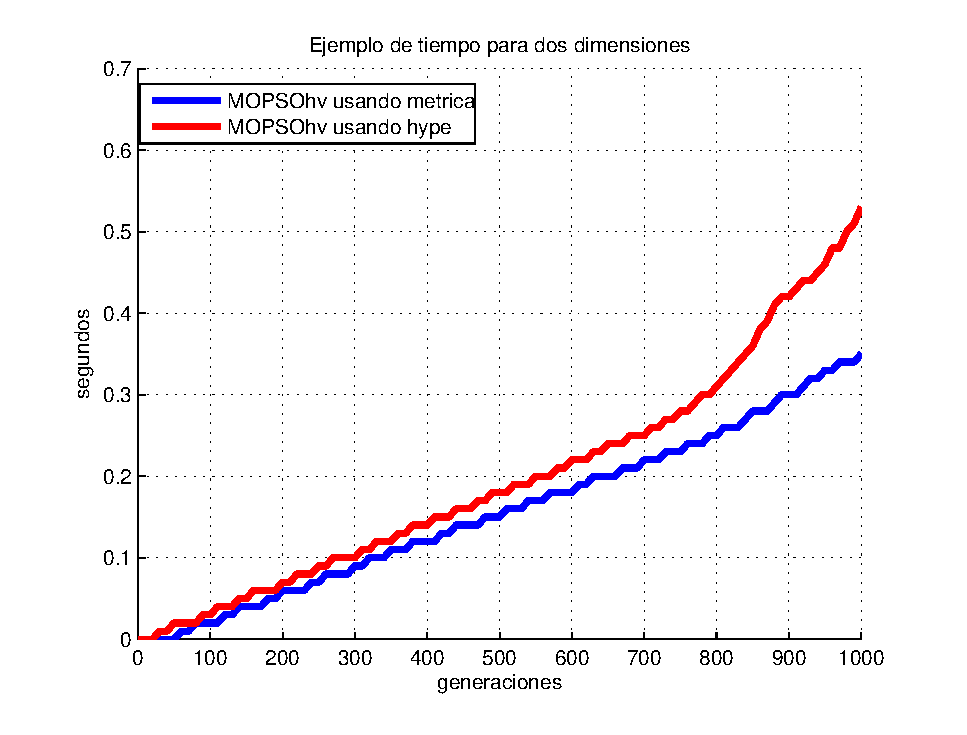
\includegraphics[scale=0.5]{Cap3/time1.eps}
    \caption[Tiempo entre MOPSOhv en dos dimensiones (a)]{Tiempo requerido en dos objetivos por el algoritmo \DIFdelbeginFL \DIFdelFL{\ref{alg:hvcont} contra 
    }\DIFdelendFL \DIFaddbeginFL \DIFaddFL{\ref{alg:MOPSOhv} usando la 
    m\'etrica completa y }\DIFaddendFL el \DIFdelbeginFL \DIFdelFL{uso
	del }\DIFdelendFL algoritmo Hype en las primeras mil generaciones.}
    \label{fig:time1}
  \end{minipage}%
  \hspace{5mm}
  \begin{minipage}{0.4\textwidth}
    \centering
    \DIFdelbeginFL %DIFDELCMD < 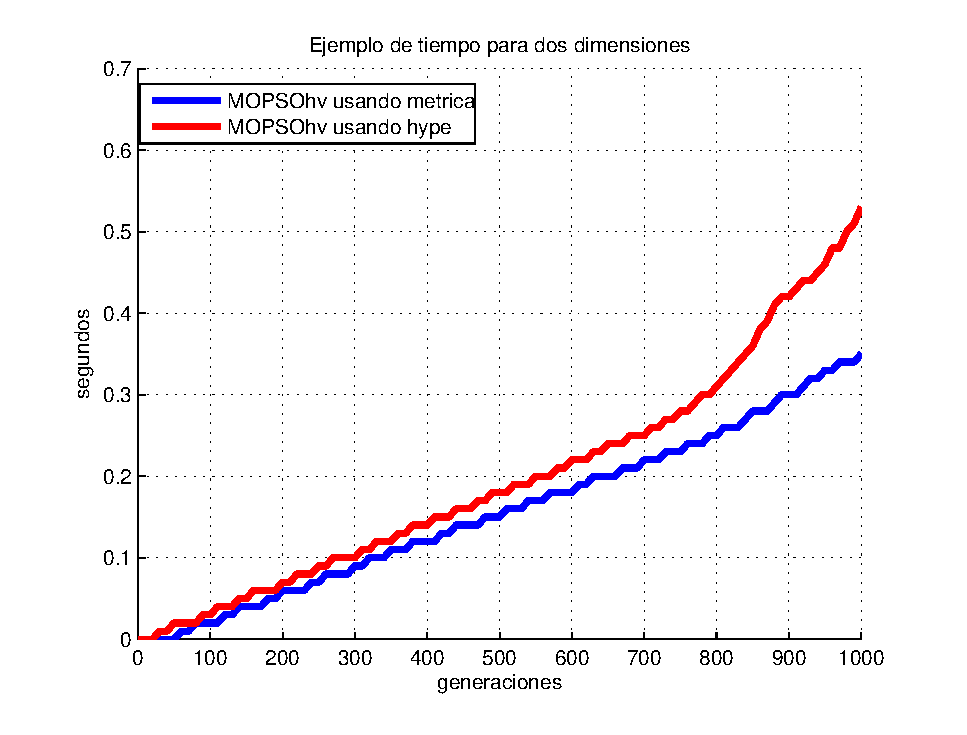
\includegraphics[scale=0.5]{Cap3/time1.eps}
%DIFDELCMD <     %%%
\DIFdelendFL \DIFaddbeginFL 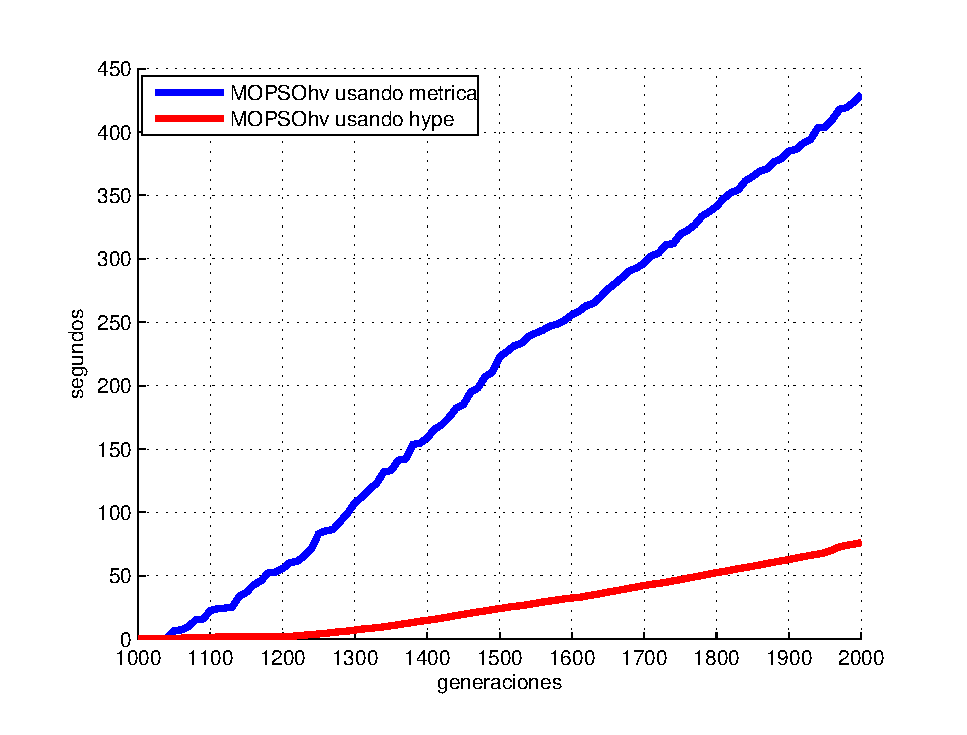
\includegraphics[scale=0.5]{Cap3/time2.eps}
    \DIFaddendFL \caption[Tiempo entre MOPSOhv en dos dimensiones (b)]{Tiempo requerido en dos objetivos por el algoritmo \DIFdelbeginFL \DIFdelFL{\ref{alg:hvcont} contra
    }\DIFdelendFL \DIFaddbeginFL \DIFaddFL{\ref{alg:MOPSOhv} usando la 
    m\'etrica completa y }\DIFaddendFL el \DIFdelbeginFL \DIFdelFL{uso
	del }\DIFdelendFL algoritmo Hype despu\'es de mil generaciones.}
    \label{fig:time2}
  \end{minipage}
  \begin{minipage}{0.4\textwidth}
    \centering
    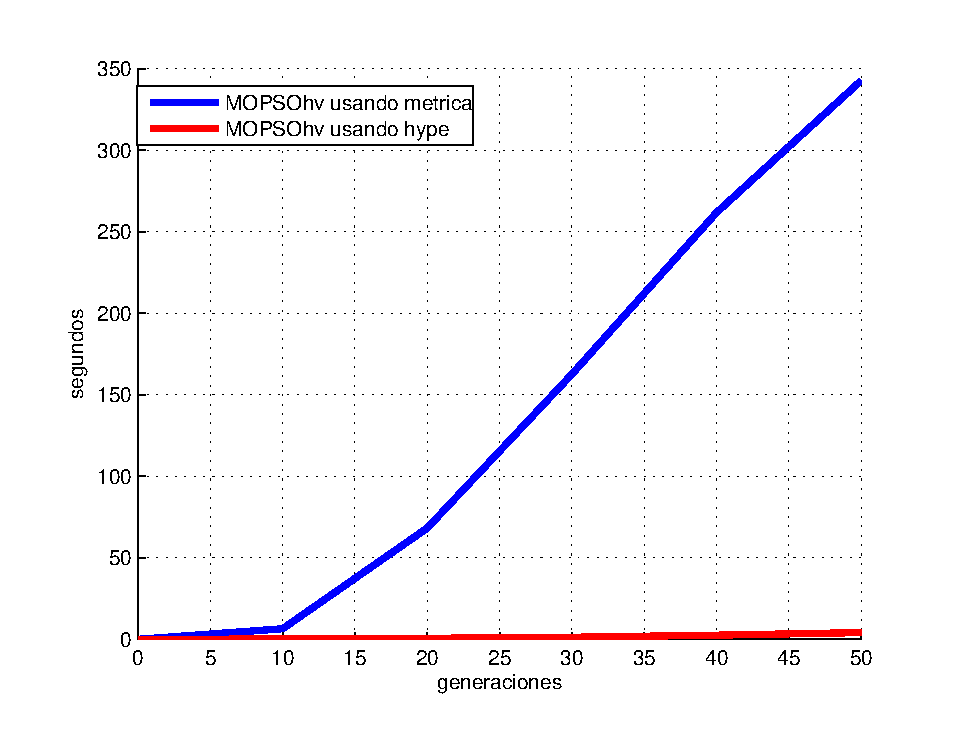
\includegraphics[scale=0.5]{Cap3/time3.eps}
    \caption[Tiempo entre MOPSOhv en tres dimensiones]{Tiempo requerido en tres objetivos por el algoritmo \DIFdelbeginFL \DIFdelFL{\ref{alg:hvcont} contra }\DIFdelendFL \DIFaddbeginFL \DIFaddFL{\ref{alg:MOPSOhv} usando la 
    m\'etrica completa y }\DIFaddendFL el \DIFdelbeginFL \DIFdelFL{uso
	del }\DIFdelendFL algoritmo Hype en las primeras 50 generaciones.}
    \label{fig:time3}
  \end{minipage}%
\end{figure}

      
     \begin{algorithm}
    \begin{algorithmic}[1]
	\IF {$dim < 3$}
	\STATE $hypeExact(C, tam_A, ref, 1, S)$
	\ELSE
	\STATE $m = 10000$        
	\STATE \DIFdelbegin \DIFdel{$l = 0$
        }%DIFDELCMD < \STATE %%%
\DIFdel{$u = ^{\max}\left\{ref\right\}$
	}%DIFDELCMD < \STATE %%%
\DIFdel{$hypeSampling(C, tam_A, l, u, m, 1, S)$
	}\DIFdelend \DIFaddbegin \DIFadd{$hypeSampling(C, tam_A, 0, ^{\max}\left\{ref\right\}, m, 1, S)$
	}\DIFaddend \ENDIF
	\RETURN $C$.
	\end{algorithmic}
	\caption{Calcular la contribuci\'on de las part\'iculas de la poblaci\'on}
	\label{alg:contMOPSOhv}
	\end{algorithm}

      \item Ordenar a la poblaci\'on en el archivo $A$ de manera descendiente conforme a su contribuci\'on al hipervolumen.

      \item Encontrar la part\'icula $w$, cuyo valor es el que menos contribuye al hipervolumen.
      \end{itemize}

\begin{enumerate}
  \item Para cada part\'icula $i$ del c\'umulo $S$, se hace lo siguiente: \\

    Actualizar la  velocidad y la posici\'on.

    \begin{itemize}

      \item Seleccionar aleatoriamente el mejor gu\'ia global ($gBest$) para la part\'icula $\mathcal{P}_i$ de un porcentaje $p$
      de las mejores part\'iculas de la poblaci\'on secundaria, la cu\'al es ordenada de manera descendente confome a su 
      contribuci\'on al hipervolumen (en nuestro caso, $p=0.01$ del porcentaje de la poblaci\'on secundaria actual). 
      En la figura \ref{fig:ordenado} se muestra un ejemplo de c\'omo ordenar la poblaci\'on del archivo de manera descendente 
      conforme a su contribuci\'on al hipervolumen. 

      \begin{figure}
      \begin{center}
	  \includegraphics[scale=0.8]{Cap3/1-15.eps}
      \end{center}
	\caption[Ejemplo de soluciones no dominadas ordenadas]{Un conjuto de soluciones no dominadas ordenadas de manera 
	descendente conforme a su contribuci\'on al hipervolumen.}
      \label{fig:ordenado}
      \end{figure}

      \item Actualizar velocidad. 

      Se utiliza la ecuaci\'on (\ref{equ:velocity}) (ver p\'agina \pageref{equ:velocity}) 
      para actualizar la velocidad de cada part\'icula $i$ del c\'umulo $S$. Para acelerar la convergencia 
      se hace uso de un factor de inercia $\omega = 0.4$, por tanto, la ecuaci\'on utilizada es la
      (\ref{equ:inercia}) (ver p\'agina \pageref{equ:inercia}). Finalmente, la ecuaci\'on queda de la siguiente 
      manera:	

       \[v^{t+1}_{i,k} = \omega \cdot v^t_{i,k} + \phi_1 \cdot rnd_1 \cdot \left(pBest^t_i - S^t_{i,k} \right) 
					    + \phi_2 \cdot rnd_2 \cdot \left(gBest - S^t_{i,k} \right),\]

      donde $\phi_1 = \phi_2 = 1$, $rnd_1 = Random(0, 1)$ y $rnd_2 = Random(0, 1)$. Cada part\'icula es evaluada 
      en cada objetivo $k$.

      \item Actualizar posici\'on. 

      Se utiliza la ecuaci\'on (\ref{equ:position}) (ver p\'agina \pageref{equ:position})
      para actualizar la posici\'on de cada part\'icula $i$ en cada objetivo $k$. La ecuaci\'on queda de la siguiente 
      manera:

      \[S^{t+1}_{i,k}=S^{t}_{i,k}+v^{t+1}_{i,k}\]

      \item Si la part\'icula $i$ se sale de la regi\'on de b\'usqueda, entonces, hay que reintegrarla utilizando los 
      l\'imites de b\'usqueda correspondientes al problema. Se multiplica la velocidad de la part\'icula $i$ por $-1$ 
      para cambiar la direcci\'on de b\'usqueda.  

      \item La mutaci\'on es una parte importante para favorecer la explotaci\'on del espacio de b\'usqueda.
      Se aplica el factor de turbulencia si se cumple que $t$ es menor a $max_{Gen} \cdot pMuta$.

    El algoritmo de c\'umulos de part\'iculas tiene una alta velocidad de convergencia. Sin embargo, esta elevada
    velocidad de convergencia puede ser perjudicial en el contexto de optimizaci\'on multi-objetivo, debido
    a que puede convergerse a un falso frente de Pareto (es decir, el equivalente de un \'optimo local en la 
    optimizaci\'on global). Para ello, introdujimos el operador de mutaci\'on que se muentra en el algoritmo \ref{alg:muta} 
    \cite{Coello04}.

    \begin{algorithm}
      \begin{algorithmic}[1]			
	\REQUIRE  Part\'icula $S_i$ para mutar, $dim$ el n\'umero de dimensiones, $max_{Gen}$ el n\'umero m\'aximo de generaciones,
	      $pMuta$ la probabilidad de mutaci\'on y $t$ la generaci\'on actual.
	\ENSURE Part\'icula \DIFdelbegin \DIFdel{$i$ }\DIFdelend \DIFaddbegin \DIFadd{$S_i$ }\DIFaddend mutada.
	\IF {$flip \left( \left( 1 - t / max_{Gen}  \right)^{5/pMuta} \right) $}
	  \STATE $wdim = random(0, dim-1)$
	  \STATE $rango = \left(u_{wdim} - l_{wdim}\right)\cdot \left(1 - t/max_{Gen} \right)^{5/pMuta}$
	  \STATE $ub = S_{i,wdim} + rango$
	  \STATE $lb = S_{i,wdim} + rango$
	  \IF{$lb < l_{wdim}$}
	    \STATE $lb = l_{wdim}$
	  \ENDIF
	  \IF{$ub > u_{wdim}$}
	    \STATE $ub = u_{wdim}$
	  \ENDIF
	  \STATE $S_{i,wdim} = random\left(lb,ub\right)$
	\ENDIF	
	\RETURN $S_i$
  \end{algorithmic}
  \caption{Operador de Mutaci\'on}
  \label{alg:muta}
  \end{algorithm}

  \end{itemize}

  \item Evaluar todas las part\'iculas de la poblaci\'on $S^t$. Se eval\'uan los valores de 
     todas las part\'iculas $i$ en cada funci\'on objetivo $k$. 

      \[p^t_{i,k} = F \left(S^t_{i,k} \right)\] 

  \item Actualizar las soluciones no dominadas en $A^t$. 

  \begin{itemize}
   \item Se insertan todas las soluciones no dominadas de $S^t$ en $A^t$, s\'olo si las soluciones no son 
  dominadas por alguna ya almacenada. Todas las soluciones dominadas por la nueva soluci\'on son eliminadas del archivo. 

  \item Si el archivo $A$ ya est\'a lleno, es decir, $nd > tam_A$. Las soluciones son reemplazadas conforme al siguiente criterio: 
  se hace uso del algoritmo \ref{alg:hvaprox} que aproxima la contribuci\'on (de la misma forma que el paso $3$). Se reemplaza la 
  part\'icula $w$, que es la que menos contribuye, con la nueva part\'icula. Se calcula la contribuci\'on y
  se encuentra otra vez a la part\'icula $w$.

  \end{itemize}

  \item Actualizar el $pBest$ de cada part\'icula $i$ en cada dimensi\'on $k$. 

  Una forma de realizarlo es si el actual $pBest_i$ es mejor que el almacenado en memoria, entonces se actualiza el $pBest^t$, de la siguiente 
  manera:

  \[pBest^t_{i,k} = S^t_{i,k}\]

  Siguiendo esta topolog\'ia no se tiene una buena interacci\'on con las dem\'as part\'iculas para generar buenas soluciones. 
  Por lo tanto, se decidi\'o actualizar el $pBest^t$ utilizando la poblaci\'on secundaria (sin considear el porcentaje $p$ de 
  las mejores   part\'iculas de esta poblaci\'on), es decir, solo se comparte informaci\'on de un porcentaje $r$ de part\'iculas 
  que pertenecen a las mejores soluciones generadas hasta el momento, las cuales ser\'an utlizadas en el entorno social del 
  algoritmo (para nuestro caso $r=1$). El $pBest^t$ se actualiza de acuerdo al algoritmo \ref{alg:contpBest}.

  \begin{algorithm}
    \begin{algorithmic}[1]
	\STATE $nttop = ((tam_A - 1) \cdot r)$
	\STATE $top = ((tam_A - 1) \cdot p)$
	\FOR {cada part\'icula $i$ hasta $tam_S$}	  
	  \STATE $j= RandomInt(top+1,nttop)$
	  \STATE $pBest^t_i = A^t_j$
	\ENDFOR
	\RETURN $pBest^t$.
	\end{algorithmic}
	\caption{Actualizar $pBest^t$}
	\label{alg:contpBest}
	\end{algorithm}

  \item Incrementar el contador de generaciones en uno.

  \[t= t + 1\]

  \item Si no se cumple el criterio de paro, retornar al paso $3$.

\end{enumerate}

\item Retornar al c\'umulo con la aproximaci\'on al frente de Pareto.

\end{enumerate}
\rule{\linewidth}{1pt}

